\documentclass[11pt]{article}
\usepackage[utf8]{inputenc}
\usepackage[T1]{fontenc}
\usepackage{amsmath,amssymb,amsthm}
\usepackage{graphicx,booktabs}
\usepackage[numbers]{natbib}
\theoremstyle{plain}
\newtheorem{theorem}{Theorem}
\newtheorem{lemma}[theorem]{Lemma}
\theoremstyle{definition}
\newtheorem{definition}{Definition}
\usepackage{hyperref}

\title{CutMix in the low-data regime}
\author{A. Author}
\date{}

\begin{document}
\maketitle

\begin{abstract}
We study CutMix when only a thousand labelled images are available. It reaches 73.2\% top-1
accuracy over \textbf{??} runs.
\end{abstract}

\section{Introduction}

% Your text. A passage taken from your notes sits between two comment lines, %%% Kind: title %%%
% and %%% end %%%: change it as you like, and leave the two lines where they are.

Mixing augmentations such as CutMix~\cite{yun2019cutmix} and mixup~\cite{zhang2018mixup} are standard; see
Definition~\ref{def:cutmix}, Lemma~\ref{lem:mixing-bound} and Figure~\ref{fig:training-loss}.

%%% Definition: CutMix %%%
\begin{definition}[CutMix]\label{def:cutmix}
Given two labelled images $(x_A, y_A)$ and $(x_B, y_B)$, CutMix~\cite{yun2019cutmix} forms
$\tilde{x} = M \odot x_A + (1 - M) \odot x_B$ and $\tilde{y} = \lambda y_A + (1 - \lambda) y_B$,
where $M$ is a binary box mask and $\lambda$ is the fraction of $x_A$ that it keeps.
\end{definition}
%%% end %%%

\section{Method}

%%% Method: Training setup %%%
We train a ResNet-50 for 200 epochs with SGD, a cosine schedule and a batch size of 256. CutMix is
applied to every batch with $\lambda \sim \mathrm{Beta}(1, 1)$.
%%% end %%%

%%% Figure: Training loss %%%
\begin{figure}[t]
  \centering
  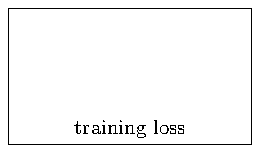
\includegraphics[width=.8\linewidth]{figures/loss.pdf}
  \caption{Training loss}\label{fig:training-loss}
\end{figure}
%%% end %%%

\section{Results}

%%% Result: CutMix at 1k images %%%
\paragraph{CutMix at 1k images.}
In our setting, CutMix reaches 73.2\% top-1 accuracy with 1k labelled images. % was: against the full set
%%% end %%%

%%% Lemma: Mixing bound %%%
\begin{lemma}[Mixing bound]\label{lem:mixing-bound}
The mixed label $\tilde{y}$ lies in the convex hull of $y_A$ and $y_B$.
\end{lemma}
%%% end %%%

\bibliographystyle{plainnat}
\bibliography{refs}
\end{document}
